\section{Experiment Setup}
To perform a normalized comparison of the LSTM and GRU cells, two models with identical hyper-parameters, but one with LSTM cell and the other with GRU cell is trained. Both of this models are setup with same number of output layers, activation function and input layers. Each of this model is composed of one input layer followed by a LSTM/GRU layer, a dropout layer and finally a dense output layer. As their is only one feature selected for this experiment, so there is only one memory unit in input layer. There are total 100 memory units in each LSTM/GRU layers with hyperbolic tangent as activation function. The summary of model is listed in Figure \ref{fig:summary}

\begin{figure}[h]
	\centering
	\subfigure[LSTM cell model]{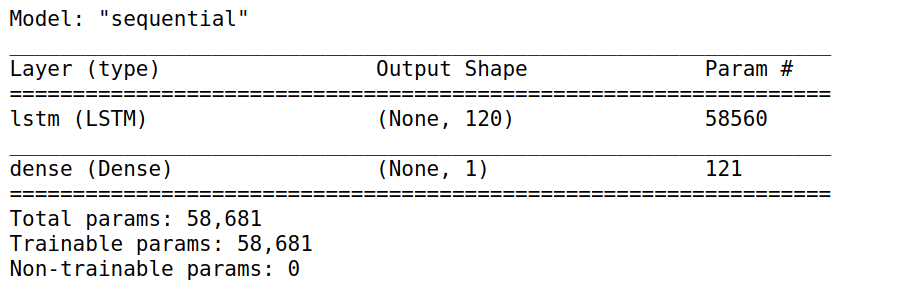
\includegraphics[width=0.8\textwidth]{Image-003.png}} 
	\subfigure[GRU cell model]{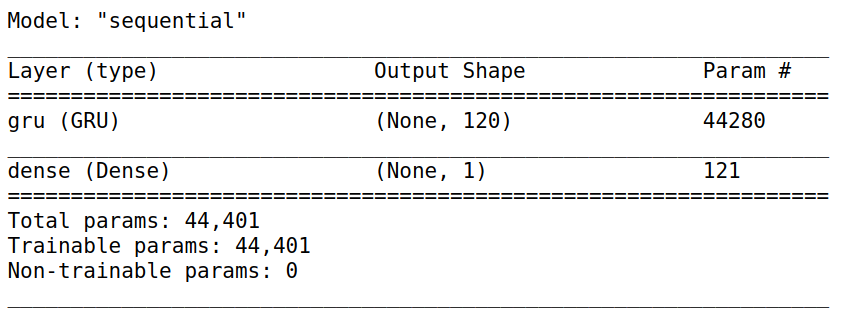
\includegraphics[width=0.8\textwidth]{Image-004.png}} 
	\caption{Model summary with (a) LSTM cell (b) GRU cell}
	\label{fig:summary}
\end{figure}

There are total of 2862 entries of data in datasets, further the total data is split into training, validation, and test sets as shown in Table \ref{table:dataset-split}. The training dataset is used to train the models where as validation dataset is used during training process to validate the values of the loss function in each epoch.

\begin{table}[h]
	\captionsetup{justification=centering}
	\caption{Training, Testing and validation data split}
	\centering
	\begin{tabular}{ c  c  c }
		\hline\hline
		Data & Date &  Data size \\ 
		\hline
		Total data & 2013-04-29 to 2021-02-27 & 2862 \\
		Training & 2013-04-29 to 2019-08-05 & 2290 \\
		Testing & 2019-08-06 to 2021-02-27 & 572 \\
		Validation & 2018-05-05 to 2019-08-05 & 458 \\
		\hline
	\end{tabular} 
	\label{table:dataset-split}
\end{table}


\section{Experiment Results}
The LSTM and GRU models are trained with an epochs value of 100 and batch size of 30 for different value of look-back period. The MAE, RMSE, CPU time, R$^2$, DA are calculated and summarized in following Tables.

\begin{table}[h]
	\captionsetup{justification=centering}
	\caption{CPU time at different look-back value }
	\centering
	\begin{tabular}{ c  c  c }
		\hline\hline
		Look Back Value & LSTM Model & GRU Model \\ 
		\hline
		4 & 11.10 sec & 8.78 sec \\
		8 & 18.98 sec & 15.14 sec \\
		12 & 33.25 sec & 26.22 sec \\
		16 & 43.79 sec & 31.50 sec \\
		\hline
	\end{tabular} 
	\label{table:result-cpu}
\end{table}

\begin{table}[h]
	\captionsetup{justification=centering}
	\caption{RMSE at different look-back value }
	\centering
	\begin{tabular}{ c  c  c }
		\hline\hline
		Look Back Value & LSTM Model & GRU Model \\ 
		\hline
		4 & 2672 & 3169 \\
		8 & 3157 & 2892 \\
		12 & 1798 & 2044 \\
		16 & 1827  & 2152 \\
		\hline
	\end{tabular} 
	\label{table:result-mae}
\end{table}
\begin{table}[h]
	\captionsetup{justification=centering}
	\caption{MAE comparison in different look-back value }
	\centering
	\begin{tabular}{ c  c  c }
		\hline\hline
		Look Back Value & LSTM Model & GRU Model \\ 
		\hline
		4 & 1150 & 1412 \\
		8 & 1589 & 1267 \\
		12 & 815 & 2227\\
		16 & 774 &  919 \\
		\hline
	\end{tabular} 
	\label{table:result-mae}
\end{table}
\begin{table}[h]
	\captionsetup{justification=centering}
	\caption{R$^2$ at different look-back value }
	\centering
	\begin{tabular}{ c  c  c }
		\hline\hline
		Look Back Value & LSTM Model & GRU Model \\ 
		\hline
		4 & 0.879 & 0.8 \\
		8 & 0.819 &  0.849 \\
		12 & 0.956 & 0.925 \\
		16 & 0.954 &  0.942 \\
		\hline
	\end{tabular} 
	\label{table:result-mae}
\end{table}
\begin{table}[h]
	\captionsetup{justification=centering}
	\caption{DA at different look-back value }
	\centering
	\begin{tabular}{ c  c  c }
		\hline\hline
		Look Back Value & LSTM Model & GRU Model \\ 
		\hline
		4 & 0.774  & 0.675\\
		8 & 0.584 &  0.737\\
		12 & 0.715 & 0.719\\
		16 & 0.697 & 0.735 \\
		\hline
	\end{tabular} 
	\label{table:result-da}
\end{table}

\section{Analysis and Discussion}
Experiments are conducted on several look-back values with epochs 100 and batch size of 30. All the metrices with different look value for both model is shown in Table \ref{table:result-cpu} to Table \ref{table:result-da}. From the results in Table \ref{table:result-cpu}, it shows that GRU trains faster than the LSTM model, which supports the conclusion made by \cite{eric2019}.


 
\begin{figure}[h]
	\centering
	\subfigure[]{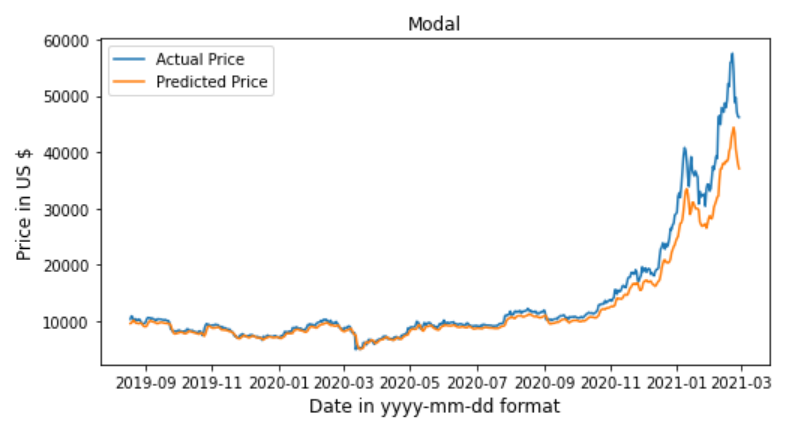
\includegraphics[width=0.8\textwidth]{Image-006.png}} 
	\subfigure[]{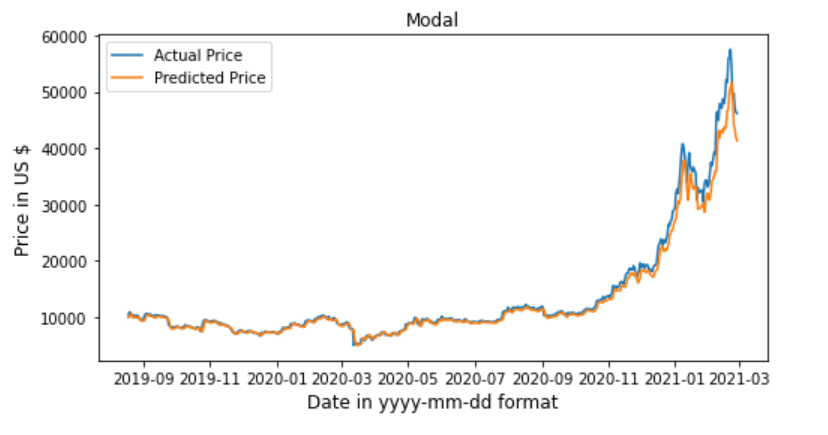
\includegraphics[width=0.8\textwidth]{Image-005.png}} 
	\caption{The actual and predicted price of Bitcoin from 2019-08-06 to 2021-02-27(a) LSTM (b) GRU}
	\label{fig:prediction}
\end{figure}